%%
%%  Example paper
%%
%%

%%%%%%%%%%%%%%%%%% Usenix style %%%%%%%%%%%%%%%%%%%%%%%%%%%%%%%%%
\documentclass[10pt,twocolumn,a4paper]{article}
\usepackage{styles/usenix-style}


%%%%%%%%%%%%%%%%%% Document %%%%%%%%%%%%%%%%%%%%%%%%%%%%%%%%%%%%%%%%%%%
% TODO: Change draft to final before submitting final version.
\usepackage[draft]{styles/ka-style}
\usepackage{xspace,ifthen,graphicx,listings}
\setlength{\marginparwidth}{2cm} % to make todonotes fit in twocolumn
\usepackage{todonotes}
\usepackage{svg}
\usepackage{dblfloatfix}
\usepackage{glossaries}

\usepackage[
   pdfauthor={Daniel Dietzler},
   pdftitle={Linux Internals},
   pdfsubject={Real-Time Linux},
   pdfkeywords={real-time, rt, linux},
   hidelinks=true
]{hyperref}

\makeglossaries

\usepackage[citestyle=numeric,style=numeric,backend=biber]{biblatex}
\addbibresource{seminar-report.bib}

\begin{document}

\newacronym{os}{OSs}{Operating Systems}
\newacronym{rt}{RT}{Real-Time}
\newacronym{rtos}{RTOSs}{Real-Time Operating Systems}
\newacronym{qos}{QoS}{Quality of Service}
\newacronym{pi}{PI}{Priority Inheritance}
\newacronym{rr}{RR}{Round Robin}
\newacronym{fifo}{FIFO}{First In First Out}
\newacronym{gedf}{GEDF}{Global Earliest Deadline First}
\newacronym{rthal}{RTHAL}{Real-Time Hardware Abstraction Layer}
\newacronym{adeos}{ADEOS}{Adaptive Domain Environemnt for Operating Systems}

% Bachelor proseminar: The title simply states your topic.
\title{Real-Time Linux}

% Master's seminar: Ideally, the title already makes clear that this is a report
% on a paper written by other researchers.
\title{%
% document class article doesn't support subtitles, let's hack them
{\normalfont \normalsize Linux Internals Proseminar}\\%
Real-Time Linux \\%
{\normalfont \normalsize \code{PREEMPT\_RT}: Making Linux Real-Time}\\%
{\normalfont \small
Karlsruhe Institute of Technology, ITEC - OS
}%
}

\author{Daniel John Dietzler}

\newcommand{\code}[1]{{\tt \small{#1}}}

\maketitle
%\draftfooter

\begin{abstract}
  There are environments like automotive and aviation where sheer throughput is not of utmost importance.
  Instead, it is necessary that processes finish within an expected time frame.
  Those systems are called \emph{real-time}.

  Writing a patch to make Linux real-time took a lot of time and effort.
  Starting in the early 2000s, a set of patches called \code{PREEMPT\_RT} made its way into Linux kernel 6.11 in late 2024.
  It involves various changes and rewrites.
  Primary efforts were targeted at making more kernel code preemptible and refactoring slow kernel applications.
  Furthermore, we will discuss performance evaluations from various studies.

  The goal of \code{PREEMPT\_RT} is to allow many projects with soft real-time needs to switch to Linux.
\end{abstract}

\section{Introduction}\label{sec:introduction}

\acrfull{rtos} are omnipresent in today's connected world.
Ranging from streaming services over networking applications to robotics ~\cite{buttazzo_hard_1997}, they all require processes to finish within a given time constraint.
In a car for instance, an airbag must deploy at the exact correct time.
Deploying too early or too late may impose significant harm to the passenger.
This is what \acrshort{rtos} are built for.
With other \acrshort{rt} applications like streaming services becoming more popular, there is an ever-growing need for simpler, yet more feature-rich \acrshort{rtos}~\cite{reghenzani_realtime_2019}.
Current solutions are good at being real-time.
However, they generally lack fundamental features such as a fully implemented network stack.
For a streaming service that is not as critical but requires modern networking, this is a problem.
Additionally, \acrshort{rtos} require developers that are specialized in that area.
Many people have experience with writing software for Linux however.
Thus, the barrier of entry becomes significantly lower.


The \code{PREEMPT\_RT} patch set involved reworking interrupt handling, replacing spin locks, and shrinking locked code sections.
Secondly, the scheduler had to be improved to reduce context switching latencies.
Additionally, a new deadline scheduler class has been introduced.
Lastly, a variety of functions in the kernel stack had to be refactored.
They are essential for daily use, but were to slow for real-time applications.
As an example we will talk about \code{printk}.

For performance, the literature suggests that \code{PREEMPT\_RT} cannot keep up with specialized Real-Time operating systems in all scenarios, especially in worst case analysis.
However, Real-Time Linux is close to being a proper hard Real-Time operating system and sufficient for most applications.

The patch does not aim to replace existing operating systems in critical applications, such as ones where life depends on.
Much more does it try to offer an alternative for soft/firm \acrshort{rt} scenarios that still should be very reactive, but for the sake of usability.
For those projects it would remove the extra burden of  \acrshort{rtos} and enable them to benefit from the broad adoption and feature-richness of Linux.
\section{Real-Time}\label{subsec:real-time}
\acrfull{rt} requires \emph{temporal determinism}.
That is, a process must terminate within a given time frame for its result to be correct~\cite{reghenzani_realtime_2019}.
Additionally, \citeauthor{buttazzo_hard_1997} names four more requirements \acrshort{rt} systems must fulfill~\cite{buttazzo_hard_1997}:

\begin{itemize}
  \item Efficiency
  \item Robustness (against peak loads)
  \item Fault Tolerance (against hardware failures)
  \item Maintainability
\end{itemize}

\acrshort{rt} approaches can be categorized into \emph{soft}, \emph{firm}, and \emph{hard} \acrshort{rt}~\cite{buttazzo_hard_1997}.

\emph{Soft \acrshort{rt}} systems suffer from \acrfull{qos} degradation.
That is, a video stream may stutter for instance.
The result however remains valid, although too late.

In \emph{firm \acrshort{rt}} systems, a late result becomes worthless.
It is, as if the result had not been computed in the first place.
A typical example for such systems is the stock exchange~\cite{reghenzani_realtime_2019}.
However, a late result does not cause any harm to the system.

Contrary to \emph{firm \acrshort{rt}}, \emph{hard \acrshort{rt}} systems do experience harm if a result is late.
Systems where human life is involved are generally considered \emph{hard \acrshort{rt}}~\cite{reghenzani_realtime_2019}.
In transportation for instance, a missed deadline can lead to the death of people.

\subsection{Real-Time in Linux}
In addition to general \acrshort{rt} properties, a patch of the Linux kernel comes with more challenges.
Required changes are so fundamental that they are very close to the core of the kernel~\cite{perlow_trenches_2021}.
Thus, the changes may not block kernel development in any way, and at the same time may be affected by frequent kernel updates~\cite{perlow_trenches_2021}.
As such, they need to be as isolated as possible.
Additionally, the patches must be as simple as possible.
The Linux kernel is already very complex~\cite{shulyupin_linux_map_2025}.
Thus, having simple patches helps with maintainability.
Furthermore, code related to the changes should also be refactored where possible in order to reduce the overall complexity~\cite{perlow_trenches_2021}.


\section{History}
The idea of \acrshort{rt} Linux has been around for over two decades ~\cite{casimiro_how_2000}.
Early on, researchers found interest in making Linux \acrshort{rt} capable.
However, initial efforts were uncoordinated and thus yielded no significant results ~\cite{perlow_trenches_2021}.
One of the first ideas was to implement a \emph{cokernel}.
While not being the final solution for Linux itself, \emph{cokernel} approaches are used by multiple \acrshort{rtos} today~\cite{reghenzani_realtime_2019}.

\subsection{Cokernel}
A \emph{cokernel} describes having a second, separate kernel besides the Linux kernel~\cite{reghenzani_realtime_2019}.
With this, both kernels get threads they can schedule processes on.
Hardware interrupts will go to a \emph{pico-kernel}.
That will forward the interrupt to the respective kernel(s)~\cite{reghenzani_realtime_2019}.
\acrshort{rt} processes will be scheduled on the \acrshort{rt} kernel.
That kernel is optimized for \acrshort{rt} applications and provides \emph{temporal determinism}.
Regular processes will be scheduled on the default, Linux kernel~\cite{reghenzani_realtime_2019}.
Having the optimal scheduler for every task by itself is highly efficient.
However, there are issues that must be dealt with.
Cokernel approaches are invasive to the Linux kernel.
Abstracting away hardware means the Linux kernel loses control and can only make weaker assumptions.
Thus, they require significant modifications~\cite{reghenzani_realtime_2019}.
With two kernels communication is expensive, so Linux applications can only be used for processes that do not have hard time constraints ~\cite{reghenzani_realtime_2019}.
Furthermore, memory swapping between the kernels can lead to page faults and dramatically impact performance~\cite{reghenzani_realtime_2019}.
Lastly, with cokernel approaches applications must still be written specifically for the \acrshort{rt} kernel.
Being different to the default Linux kernel, there are other system calls that are available and need to be used.
This requires specialized developers and multiple versions of the same application~\cite{reghenzani_realtime_2019}.

\begin{figure*}[ht]
  \centering
  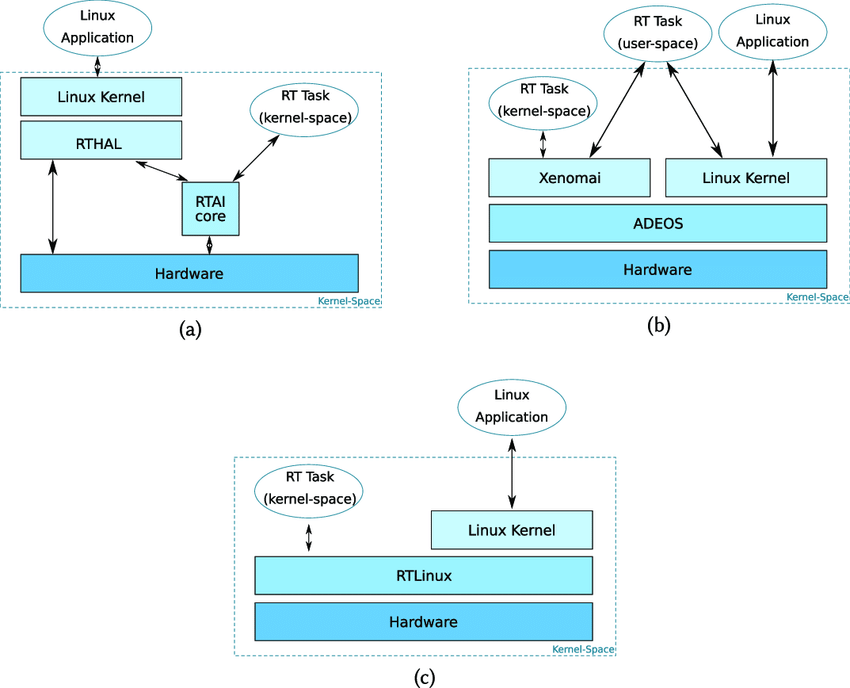
\includegraphics[scale=.50, clip]{assets/cokernel.png}
  \caption{Cokernel approaches. (a) RTAI, (b) Xenomai, (c) RTLinux~\cite{reghenzani_realtime_2019} \label{fig:cokernel}}
\end{figure*}
Nonetheless, cokernel approaches are broadly represented in today's \acrshort{rtos} landscape.
\emph{RTAI}~\cite{rtai-docs}, \emph{Xenomai}~\cite{xenomai-docs}, and \emph{RTLinux}\footnote{Note that this is \emph{not} \acrlong{rt} Linux.}~\cite{rtlinux}. are all popular examples of modern \acrshort{rtos} building on cokernels as can be seen in \autoref{fig:cokernel}~\cite{reghenzani_realtime_2019}.
In all cases, the Linux kernel sits on top of a \acrshort{rt} (pico-)kernel.
RTAI uses a pico-kernel called \emph{RTAI core} that schedules \acrshort{rt} kernel space processes.
Then, on top of that there is the \acrfull{rthal} that provides the expected interfaces for the Linux kernel.

Xenomai uses a common pico-kernel called \acrfull{adeos}.
It provides an abstraction layer for both the Xenomai kernel that schedules \acrshort{rt} processes but also the Linux kernel.

Lastly, RTLinux only uses one additional kernel -- called \emph{RTLinux} -- that provides the hardware abstraction for the Linux kernel as well as \acrshort{rt} scheduling for respective processes.
\newline

\noindent All the uncoordinated efforts towards making Linux \acrshort{rt} led to chaos in 2004~\cite{perlow_trenches_2021}.
At that point, a loose team started to form around Molnar~\cite{perlow_trenches_2021}.
Within a few months the team built a proof of concept~\cite{perlow_trenches_2021}.
While being "far from a maintainable and production-ready solution"~\cite[Gleixner]{perlow_trenches_2021}, it showed that the idea a \acrshort{rt} Linux was feasible~\cite{perlow_trenches_2021}.
Originally planned for 2018~\cite{lf:history}, \code{PREEMPT\_RT} made it into the LTS kernel in 2024 with kernel version 6.11~\cite{lf:versions}.

\section{Kernel Patch: \code{PREEMPT\_RT}}
In order to make the Linux kernel \acrshort{rt}-capable, many fundamental changes had to be made.
All of those had been grouped in a set of patches called \code{PREEMPT\_RT}.
Firstly, scheduler improvements were necessary in order to reduce latencies and achieve tighter timing~\cite{mckenney_realtime_2005}.
New kernel analytics tools helped identifying code sections that could improved, while also uncovering new bugs in Linux~\cite{reghenzani_realtime_2019}.
On \acrshort{rtos} context switches happen more frequently due to the nature of \acrshort{rt} applications.
That is, because in order to guarantee turnaround times, low priority processes need to be preempted if a high priority process comes in~\cite{buttazzo_hard_1997}.
This directly leads to the need to reduce the amount of non-preemptible kernel code~\cite{reghenzani_realtime_2019}.
Part of the Linux kernel that was non-preemptible were interrupt handlers \cite{reghenzani_realtime_2019}.
That is why, in the following, we start by looking at interrupts in \autoref{subsec:interrupts}.
After that, we will be going over locking mechanisms and the introduction of a new lock with \code{PREEMPT\_RT} in \autoref{subsec:locking}.
Then, we will discuss preemption as a central aspect of \acrshort{rt} systems, followed by a section on high resolution timers in \autoref{subsec:hr-timers}.
Those timers enable better scheduling, which is crucial for \acrshort{rt}.
Lastly, \autoref{subsec:scheduler} discusses the changes to the scheduler.

\subsection{Interrupts}\label{subsec:interrupts}
Interrupt handler are subdivided into a \emph{soft} and \emph{hard} part.
The hard interrupt request handler responds immediately and takes care of the most important operations~\cite{reghenzani_realtime_2019}.
Later, the soft interrupt request handler does additional processing~\cite{reghenzani_realtime_2019}.
By default, soft interrupt request handlers also run in the context of the interrupt service routine~\cite{lf:irq}.
By being part of the interrupt service routine, hardware interrupts are disabled~\cite{lf:irq}.
This makes soft interrupt request handlers non-preemptible~\cite{lf:irq}.
With \code{PREEMPT\_RT}, a flag allows soft interrupt request handlers to run in a threaded context instead, making them preemptible~\cite{reghenzani_realtime_2019, lf:irq}.
By default, that thread will be scheduled with \acrfull{fifo} and a high priority of 50~\cite{lf:irq}.

For interrupt handlers that -- under no circumstances -- may run in a threaded context, there is an extra flag to disable this behavior per handler~\cite{lf:irq}.
Generally, one should be careful with this flag though.
It will be prone to deadlocks, making the development of those handlers harder~\cite{mckenney_realtime_2005}.
For instance, another preempted thread could have a lock on a resource that is required by the soft interrupt request handler.
If the handler cannot be preempted by e.g. a timer at some point it will wait for that lock to free forever, hogging CPU resources.
Also, in order to reduce the amount of non-preemptible code, this flag should be used as rarely as possible.
One example for forcing a handler to run in the interrupt context are per-CPU timer interrupts.
With their tight schedules and low-level relevance, they qualify for being non-preemptible~\cite{mckenney_realtime_2005}.

\subsection{Locking}\label{subsec:locking}
In order to further reduce the amount of non-preemptible code, locked, critical sections have been narrowed~\cite{mckenney_realtime_2005}.
Additionally, locking mechanisms have been reworked and a new lock got added.

In the kernel, many locks used to be spinlocks ~\cite{lf:sleeping-spinlocks}.

\subsubsection{Changes}
With \code{PREEMPT\_RT}, all \code{spinlock\_t} kernel spinlocks have been replaced by \code{rt\_mutex} by default.

\code{rt\_mutex} implements \emph{priority inheritance} to avoid the problem of \emph{priority inversion}~\cite{rostedt_rtmutex_2017}.
That is, one process having a higher priority but waiting for a lower priority process to free a lock.
In that scenario, the higher priority process cannot run until the lower priority process finishes, even though it has a higher priority.
For \code{rt\_mutex}, \acrfull{pi} is implemented by giving each process a \acrshort{pi} \emph{rbtree}, depicting the dependencies of the waiters.
A \acrshort{pi} rbtree of a process stores the top waiter, that is the process with the highest priority currently waiting for that lock, of every lock that is held by that process ~\cite{rostedt_rtmutex_2017}.
The dependencies of processes and their locks is called a \acrshort{pi} chain~\cite{rostedt_rtmutex_2017}.
\lstset{basicstyle=\small}
\begin{lstlisting}[caption={Example from~\cite{rostedt_rtmutex_2017}}]
Processes:  A, B, C, D, E
Mutexes:  L1, L2, L3, L4
\end{lstlisting}
\begin{figure}[htb]
  \centering
  \includesvg[scale=.8]{assets/pi_chain.svg}
  \caption{Example from~\cite{rostedt_rtmutex_2017}}
\end{figure}
Translating this example into a \acrshort{pi} chain results in this:
\begin{lstlisting}[caption={Simple \acrshort{pi} chain~\cite{rostedt_rtmutex_2017}}]
E->L4->D->L3->C->L2->B->L1->A
\end{lstlisting}
By adding another process $F$ and a mutex $L5$ with the dependencies as follows
\begin{lstlisting}[caption={Second \acrshort{pi} chain~\cite{rostedt_rtmutex_2017}}]
F->L5->B->L1->A
\end{lstlisting}
we can see multiple chains merged together:
\begin{lstlisting}[caption={\acrshort{pi} chain~\cite{rostedt_rtmutex_2017}}]
E->L4->D->L3->C->L2-+
                    |
                    +->B->L1->A
                    |
              F->L5-+
\end{lstlisting}
Based on this chain, priorities can be changed in order to avoid priority inversion:
A process further right in the chain must always have a priority equal to or higher than processes on the left of it~\cite{rostedt_rtmutex_2017}.
\newline

\noindent This change aims to drastically reduce the amount of spinlocks in the kernel code, making more sections preemptible overall~\cite{lf:sleeping-spinlocks}.
However, instead of renaming the type, it was decided to change its implementation depending on whether \code{PREEMPT\_RT} is enabled or not.
This has been done to avoid changing too much kernel code and making pull requests unreviewable~\cite{reghenzani_realtime_2019}.
We argue that this comes at the expense of non-intuitive kernel code.
If \code{PREEMPT\_RT} is enabled, \code{spinlock\_t} acts as a \code{rt\_mutex}, otherwise it acts as a normal spinlock~\cite{mckenney_realtime_2005}.
In case there is need for a genuine spinlock that always behaves as such, \code{raw\_spinlock\_t} can used instead~\cite{mckenney_realtime_2005, chyyuu_github_2017}.
Predominantly, actual spinlocks are necessary in interrupt handlers that do not run in a threaded context and shall not be preempted.


\subsection{Preemption}\label{subsec:preemption}
In order to fulfill \acrshort{rt} requirements, preemption is of utmost importance.
Before the \code{PREEMPT\_RT} patch there have been three preemption modes in the Linux kernel: \code{PREEMPT\_NONE}, \code{PREEMPT\_VOLUNTARY}, and \code{PREEMPT}~\cite{lf:preemption,kernel_preemption_modes}.

As the name suggests, \code{PREEMPT\_NONE} does not have any additional preemption points~\cite{kernel_preemption_modes}.
The only scenarios where preemption happens are for system call returns and interrupts.
This is the traditional Linux, which emphasizes on throughput.

With \code{PREEMPT\_VOLUNTARY}, some explicit preemption points are added to the kernel code~\cite{kernel_preemption_modes}.
Specifically \code{might\_sleep()} and \code{might\_sleep\_if()} calls become preemption points~\cite{day_re_2007}.
\emph{Voluntary Kernel Preemption} is on regular Linux desktops ~\cite{mckenney_realtime_2005}.

In \code{PREEMPT} mode, all kernel code that is not running in a critical section becomes preemptible~\cite{kernel_preemption_modes}.
That is, sections that are not covered by a mutex.
This reduces the kernel latency and is thus used in low-latency desktop applications.~\cite{mckenney_realtime_2005}.
However, this does not make Linux a \acrshort{rtos}.
\newline

\noindent The \code{PREEMPT\_RT} patch added two new preemption modes to the Linux kernel, namely \emph{Preemptible kernel (basic \acrshort{rt})} and \code{PREEMPT\_RT}, which is named similar to the patch~\cite{lf:preemption,kernel_preemption_modes}.

\emph{Preemptible kernel (basic \acrshort{rt})} is mainly intended for debugging purposes.
Its only difference in comparison to \code{PREEMPT} is that it forces the use of threaded soft interrupt handlers, if not explicitly disabled for that handler~\cite{lf:preemption}.
Threaded interrupt handlers are preemptible and make up a significant part of the \code{PREEMPT\_RT} patch.

Finally, the \code{PREEMPT\_RT} kernel mode actually constitutes \acrshort{rt} Linux.
In addition to \code{PREEMPT}, most critical sections are preemptible as well, making the Linux kernel broadly preemptible~\cite{lf:preemption}.
Furthermore, threaded interrupt handlers are enforced, too.
Substituting spinlocks with \code{rt\_mutex}es as well as breaking up large non-preemptible sections -- as discussed in \autoref{subsec:locking} -- lastly give Linux its \acrshort{rt} behavior~\cite{lf:preemption}.

\begin{figure}[htb]
  \centering
  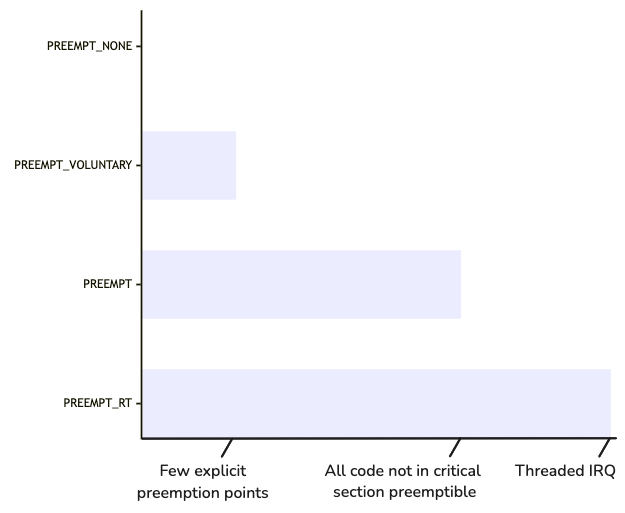
\includegraphics[scale=.36, clip]{assets/preemption_modes.png}
  \caption{Relevant Preemption Modes}
\end{figure}

\subsection{High Resolution Timers}\label{subsec:hr-timers}
Among the most important aspects of a \acrshort{rtos} is a tight scheduler that can very quickly switch between processes ~\cite{reghenzani_realtime_2019}.
This comes down to two things; (1) preemption and (2) a "good" \acrshort{rt} scheduler.
We have already seen (1) in \autoref{subsec:preemption}.
In order to achieve (2), there is one more part required; better timers.
Before \code{PREEMPT\_RT}, system timers could only be set with the precision of the \emph{tick rate}~\cite{reghenzani_realtime_2019} due to an absence of high resolution timers in hardware in the early days of Linux.
With \code{PREEMPT\_RT}, \acrshort{rt} Linux introduces \emph{high resolution timers}~\cite{lf:timers}.
For the first time in Linux, they allow nanosecond-granular timers ~\cite{reghenzani_realtime_2019}.
This allows to e.g. configure finer timer interrupts, resulting in a more reactive scheduling.
Threads do not take up unnecessary time before they get preempted even though they already finished computing.

\subsection{Scheduler}\label{subsec:scheduler}
A typical scheduler can have multiple \emph{scheduler classes} based on which it evaluates scheduling decisions.
Each class hereby has its own scheduling algorithm and rules.
Linux has two realtime scheduler classes; the \emph{(POSIX) realtime scheduler} and the \emph{deadline scheduler}~\cite{bristot_de_oliveira_deadline_2018}.
Firstly, the \emph{realtime scheduler class} implements \code{SCHED\_FIFO} and \code{SCHED\_RR}~\cite{lf:scheduler}.
Both schedule processes based on their fixed priority~\cite{lf:scheduler,de_oliveira_timing_2016}.
In \acrfull{fifo} fashion, for processes of the same priority, the process that arrived first in the queue of processes to be scheduled will run as long as possible before any other process gets scheduled with \code{SCHED\_FIFO}.
Contrarily, \code{SCHED\_RR} uses \acrfull{rr}.
It will cycle through all processes of the highest priority, giving each process time slices ~\cite{bristot_de_oliveira_deadline_2018}.

Secondly, the \emph{deadline scheduler class} only has one scheduling policy: \code{SCHED\_DEADLINE}~\cite{bristot_de_oliveira_deadline_2018}.
That policy implements the \acrfull{gedf} algorithm~\cite{lelli_deadline_2016}.
Instead of making scheduling decisions based on (fixed) priorities, the process with the earliest deadline is considered 'most important' and will be scheduled first~\cite{bristot_de_oliveira_deadline_2018}.
Processes scheduled using the \emph{deadline scheduler class} can preempt other processes scheduled by the \emph{realtime scheduler} based on \acrshort{fifo} or \acrshort{rr}~\cite{lf:scheduler}.

Deadline scheduling is simple for both, the user to work with, and implementing a scheduler~\cite{bristot_de_oliveira_deadline_2018}.
A user does not need to think about priorities.
Especially, they do not need to think about other processes, and how those might impact their process ~\cite{bristot_de_oliveira_deadline_2018}.
The user simply has to say when the process needs to have finished, and the scheduler by definition will try to make it work as can be seen in the following.

For the implementation of the scheduler, there is no need to analyze any other processes, that is evaluate priorities, consider priority inheritance, follow complex scheduling policies~\cite{bristot_de_oliveira_deadline_2018}.
It has to always schedule the process with the earliest deadline.
This way, all deadlines are trivially held -- assuming they were possible to meet in the first place~\cite{bristot_de_oliveira_deadline_2018}.
This approach also ensures the minimal amount of context switches ~\cite{bristot_de_oliveira_deadline_2018}.
Only when a process with an earlier deadline than the currently scheduled process comes in, the scheduler needs to reschedule and triggers a context switch.

\begin{figure}[htb]
  \centering
  \includesvg[scale=.7]{assets/deadline_scheduling.svg}
  \caption{Deadline scheduling}
\end{figure}

However, this approach also comes with downsides.
Inherently, deadline scheduling does not deliver minimal response times ~\cite{bristot_de_oliveira_deadline_2018}.
Furthermore, "it is possible to face a domino effect"~\cite[Daniel Bristot de Oliveira]{bristot_de_oliveira_deadline_2018}.
Assuming the process with the earliest deadline has a deadline that is unreachable because it is too soon.
The scheduler will still schedule that process and spend CPU cycles on it, even though it can never finish in time.
This can cause the next process to not meet its deadline as well, even though it could have reached it, if it was scheduled first~\cite{bristot_de_oliveira_deadline_2018}.
Thus, such an unmeetable deadline can trickle down to all subsequent processes and cause an entire batch to be late.


\subsection{Kernel Library}
In addition to fundamental changes to the scheduler, locking, and preemption mechanisms, there were also libraries used in the kernel that needed updating and have a more noticeable impact on users.
Some essential utility implementations in the kernel had latencies too high for a \acrshort{rt} application~\cite{edge_discussion_2022}.
As an example, we will be discussing \code{printk}, the kernel equivalent to \code{printf}.

\subsubsection{\code{printk}}
According to \citeauthor{edge_discussion_2022}, \code{printk}'s latency used to be "unacceptably high" for \acrshort{rt} Linux~\cite{edge_discussion_2022}.
Additionally, a general rework of the library has been long overdue anyways ~\cite{edge_discussion_2022}.
Lastly, \code{printk} used to use a global kernel lock, increasing the latency of the entire system further~\cite{gleixner_printk_2024}.
An initial suggestion to make \code{printk} work in \acrshort{rt} Linux essentially disabled \code{printk} if \code{PREEMPT\_RT} is enabled~\cite{mladek_printk_2022}.
Linus Torvalds considered this inviable~\cite{torvalds_initial_2022}, leading to a new implementation.

\paragraph{Changes.}
Primarily, the global kernel lock has been replaced.
Instead, there are now per-console kernel threads which take care of flushing normal priority messages to the console~\cite{gleixner_printk_2024}.
This directly leads to the second addition; priorities.
Every printing process has a priority and needs to check, each time it prints a byte, if it can still print or if there is a process with a higher priority waiting~\cite{edge_discussion_2022}.
\emph{panic} messages can do a \emph{hostile takeover} of a console if necessary.
That is, forcefully taking over a console that is currently in use.
That allows to get as many information to the user before the system or process dies completely~\cite{edge_discussion_2022}.
To decide which console to print to, the \code{printk} implementation is now differentiating \emph{safe} and \emph{unsafe} consoles.
For instance, a console becomes \emph{unsafe} if it has experienced a hostile takeover before~\cite{kernel_development_community_console}.
In case of a \emph{panic}, the process will always try to print to a safe console to increase its chances of getting any logs printed before it dies~\cite{gleixner_printk_2024}.
If there is none available, the process will try its final flush on an unsafe console and "Hope and pray"~\cite{kernel_development_community_console}.
That means there is no guarantee if any characters will be printed or not.

\section{Discussion}
\subsection{RTOS vs \code{PREEMPT\_RT}}
Traditional \acrshort{rtos} are highly specialized in their domain.
Specifically, they do not have a standard Linux kernel.
That comes with a variety of difficulties.
Firstly, the feature set of those specialized kernels is much reduced.
For instance, Xenomai has a much reduced network stack with only a partial, simple implementation of TCP~\cite{xenomai_network_2024}.

Secondly, given Linux's popularity, there are a lot of user space libraries built for Linux.
This allows developers to more easily build new applications, compared to \acrshort{rtos} where many functions need to be implemented from the ground up.
The latter is a non-trivial task and requires much more time and money.

Thirdly, having non-popular libraries and a non-standard kernel, specialized developers are needed.
Most low-level developers know Linux, but only a few are actually experienced with \acrshort{rtos} such as RTAI.

Lastly, Linux supports a variety of architectures.
This, however, is not the case with \acrshort{rtos}.
Although, we see improvements with \acrshort{rtos} becoming more compatible.
Xenomai for instance has full support for x86 by now~\cite{xenomai_supported}.
Also, the nature of cokernel approaches implies having to write an abstraction layer for every Linux kernel version.
This is because invasive modifications of the Linux kernel are necessary, which break with kernel updates ~\cite{reghenzani_realtime_2019}.
This implies \acrshort{rtos} are always behind the latest kernel version~\cite{xenomai-docs}.
\newline

\noindent The \code{PREEMPT\_RT} patch on the other hand suffers from infrastructural issues.
The working group around the patch lacks resources ~\cite{perlow_trenches_2021}.
As is with many open source projects, funding is a problem here, too~\cite{perlow_trenches_2021}.

Secondly, it also lacks long-term commitment, both from the developers as well as supporters ~\cite{perlow_trenches_2021}.
If there is not enough money to pay more developers, developers are less likely to commit (lots of) their time to it.


\subsection{Hard RTOS?}
Linux is a huge and extremely complicated codebase.
Additionally, it can be run on a variety of different systems.
As such, modelling the Linux runtime environment for formal proofs is virtually impossible~\cite{reghenzani_realtime_2019}.
This however implies, that \code{PREEMPT\_RT} cannot ever reach the same reliability level as some of the \acrshort{rtos}.
The guarantees that can be made about \code{PREEMPT\_RT} do not have a chance to be as strong as those that can be made about \acrshort{rtos}~\cite{reghenzani_realtime_2019}.
The \acrfull{lf} project \emph{ELISA}~\cite{elisa_2025} aims to validate the patch, but a 100\% validation seems impossible~\cite{perlow_trenches_2021}.
Gleixner explains that \acrshort{rt} Linux never aimed to be highly specialized~\cite{perlow_trenches_2021}.
The most critical applications that require formal validation and an absolute certainty should not rely on \code{PREEMPT\_RT}.

This also puts \acrshort{rt} Linux in an odd position when trying to sort it into the \emph{soft}, \emph{firm}, and \emph{hard} hierarchy.
As mentioned before in \autoref{subsec:real-time}, \emph{soft} \acrshort{rt} systems can miss deadlines without any bad consequences.
\emph{firm} systems do not cause any damage to people or systems if a result runs late, but their result becomes worthless.
Lastly, \emph{hard} \acrshort{rtos} do not tolerate any late results.
If a computation does not meet a deadline, people or systems can be damaged.

The \code{PREEMPT\_RT} patch provides stronger guarantees than \emph{firm} and especially \emph{soft} \acrshort{rt} systems require~\cite{reghenzani_realtime_2019}.
While doing a lot to also meet \emph{hard} \acrshort{rt} requirements, the community does not consider \acrshort{rt} Linux to be a \emph{hard} \acrshort{rt} system~\cite{barbieri_rt-linux_rtos}.
Companies with \emph{hard} \acrshort{rt} use cases have not considered switching to \code{PREEMPT\_RT} and are unlikely to do so anytime soon~\cite{reghenzani_realtime_2019}.
This is primarily due to the lack of formal verifiability~\cite{reghenzani_realtime_2019}.
In conclusion, \code{PREEMPT\_RT} sits somewhere in between \emph{firm} and \emph{hard} \acrshort{rtos}.
The terms \emph{95\% hard \acrshort{rt} systems} and \emph{probabilistic hard \acrshort{rt} systems} may be used to describe \acrshort{rt} Linux instead~\cite{reghenzani_realtime_2019}.
The idea of \emph{probabilistic hard \acrshort{rt} systems} is to use statistical theories to describe the likelihood of environmental factors and based on that, obtain formal validation~\cite{reghenzani_realtime_2019}.
However, that is not a broadly accepted term yet and realistically \code{PREEMPT\_RT} is not a \emph{hard} RTOS~\cite{reghenzani_realtime_2019} -- which it does not aims to be~\cite{perlow_trenches_2021}.

\subsection{Performance}

\begin{figure*}[htb]
  \centering
  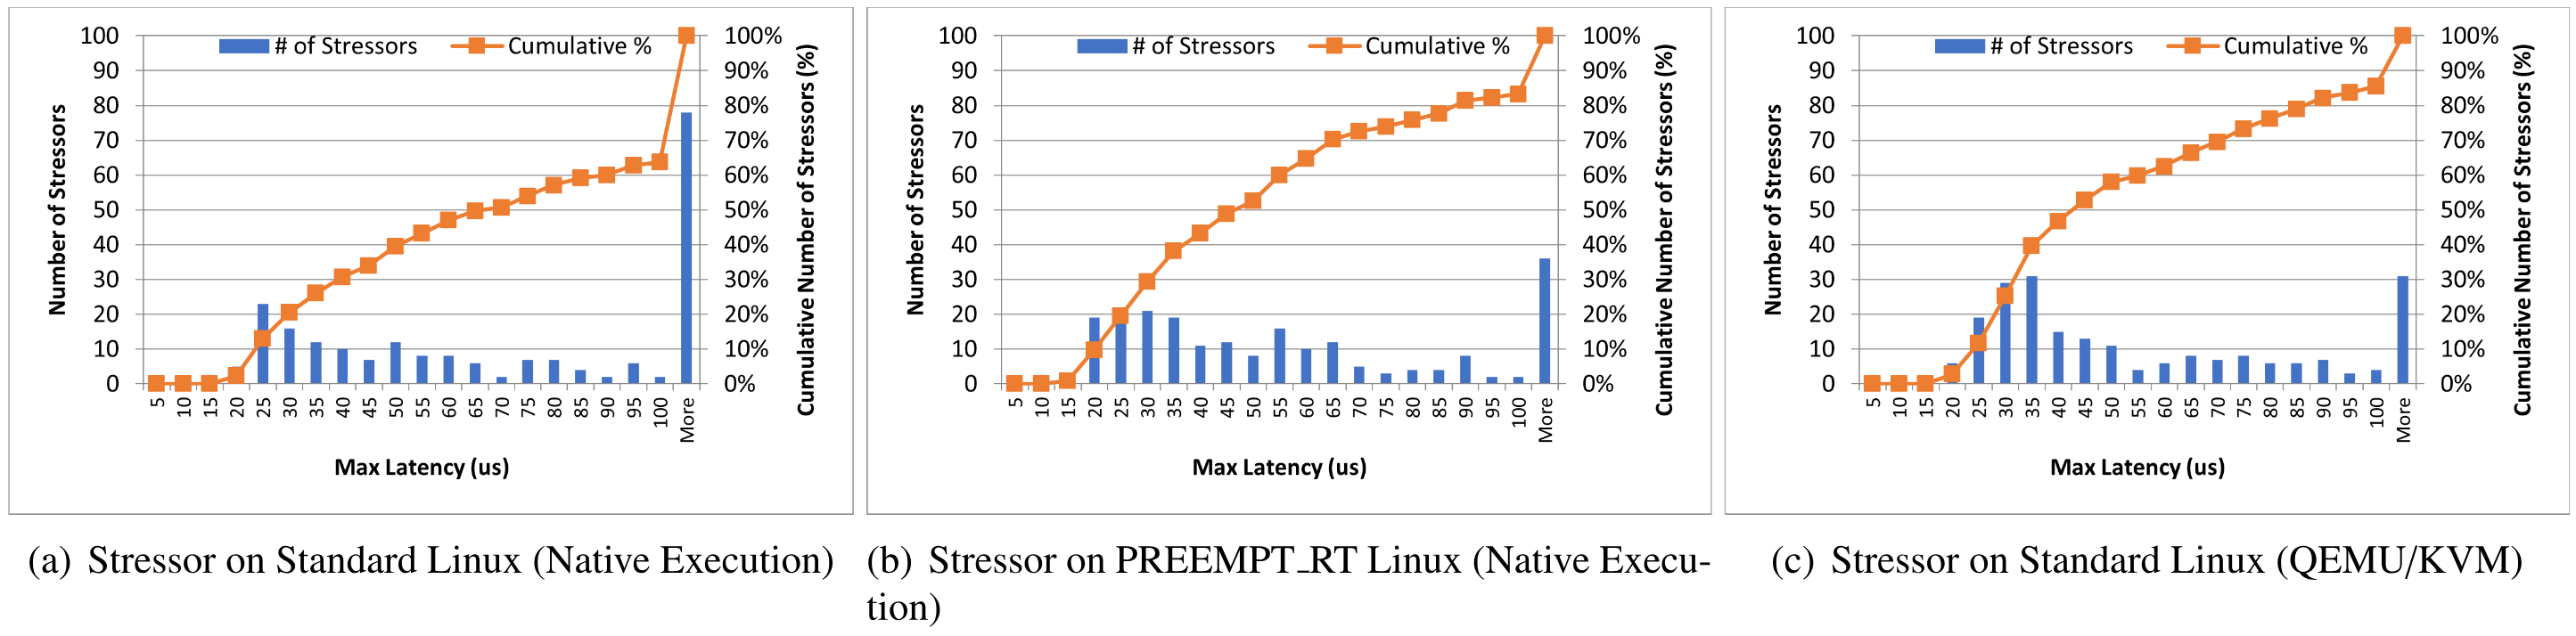
\includegraphics[scale=.162]{assets/preemptrt_latencies.png}
  \caption{Latencies under load~\cite{li_performance_2023}}
  \label{fig:latencies}
\end{figure*}

\citeauthor{reghenzani_realtime_2019} summarized various articles measuring \code{PREEMPT\_RT} and comparing it to other \acrshort{rtos}~\cite{reghenzani_realtime_2019}:
\code{PREEMPT\_RT} showed a scheduling latency that maxed out at $10 - 15\mu s$, overall being similar to the RTOS $\text{LITMUS}^{\text{RT}}$~\cite{litmusrt}.
In CPU-bound workloads, it actually outperformed $\text{LITMUS}^{\text{RT}}$ in latency speed ($\sim 17\mu s$ vs. $\sim 47\mu s$).

Compared to RTAI and Xenomai, the Linux kernel patch does not quite reach the same task switching speeds.
While the other \acrshort{rtos} manage averages of $<1\mu s$, \code{PREEMPT\_RT} does not make it below $1 \mu$~\cite{reghenzani_realtime_2019}.
In worst case scenarios, \code{PREEMPT\_RT} manages to keep up with RTAI at around $20\mu s$, but being vastly outperformed by Xenomai with a worst case task switching speed of $\sim 2\mu s$.

As also noted by \citeauthor{reghenzani_realtime_2019}, this shows that \acrshort{rtos} specialization is still noticeable, and especially in worst case scenarios \code{PREEMPT\_RT} cannot keep up~\cite{reghenzani_realtime_2019}.
Yet, Linux is a \acrfull{gpos} after all, trying to make the stretch between high throughput and reactive \acrshort{rt} behavior.

While the paper from \citeauthor{reghenzani_realtime_2019}~\cite{reghenzani_realtime_2019} only has outdated data, \citeauthor{li_performance_2023}~\cite{li_performance_2023} conducted throughput measurements on recent software and hardware themselves.
They were running on a Raspberry Pi 4 with four cores and Ubuntu 20.04 LTS.
We find this still quite representable, especially kernel 5.4 is -- although still quite dated by now -- much more recent than 2.6.33 from the comparison in~\cite{reghenzani_realtime_2019}.

\code{PREEMPT\_RT} can lead to a 29\% throughput degradation when using all four cores, with only a 6\% degradation in singe core loads ~\cite{li_performance_2023}.
This is similar to the dated results presented in~\cite{reghenzani_realtime_2019} where \citeauthor{reghenzani_realtime_2019} saw a degradation of up to 35\% in multi core loads.
Especially for a file copy workload the authors have seen a decrease in throughput with an increase in core counts when using \code{PREEMPT\_RT}~\cite{li_performance_2023}.
This suggests that accessing a single device is not scalable with the kernel patch~\cite{li_performance_2023}.
Furthermore, they ran a Linux kernel in a QEMU/KVM VM on top of the Linux host with \code{PREEMPT\_RT} enabled.
They saw that running non-\acrshort{rt} processes in that VM yielded a 40\% higher throughput rate compared to running it on the \code{PREEMPT\_RT}-enabled host~\cite{li_performance_2023}.
As can be seen in \autoref{fig:latencies}, the impact of the VM on the overall system latency is also minimal.
There is a slight variation in the lower latencies between (b) and (c), with a reduction in latencies on the upper end in (c)~\cite{li_performance_2023}.
Thus, given the minimal virtualization overhead, this could be a valid mitigation strategy~\cite{li_performance_2023} to feasibly run non-\acrshort{rt} tasks with \code{PREEMPT\_RT} enabled.

\section{Conclusion}
The idea of making Linux \acrshort{rt}-capable has been around for a long time.
20 years ago combined efforts were started being put into \code{PREEMPT\_RT}, the Linux kernel patch that made it into the kernel in late 2024.
\code{PREEMPT\_RT} cannot be considered a \emph{hard} \acrshort{rtos}.
This is primarily due to the Linux kernel being very large and Linux' primary use case being a \acrshort{gpos}.
However, \code{PREEMPT\_RT} aims at being a viable solution for many \emph{soft}/\emph{firm} \acrshort{rt} use cases.
Contrary to other \acrshort{rtos}, developing on the Linux kernel allows to use many quality of life features and reduces friction in developing applications.
In order to make \code{PREEMPT\_RT} happen, many changes were necessary:
Primarily, non-preemptible sections have been reduced, specifically interrupt service routines.
Additionally, locking updates were done to further make code sections in the kernel preemptible.
Furthermore, the scheduler has been updated and a new scheduling policy got introduced, alongside high resolution timers.
Lastly, many kernel library programs were too slow for \acrshort{rt} applications.
Those have been refactored, as for instance \code{printk}.
Ultimately, \code{PREEMPT\_RT} is unlikely to replace \acrshort{rtos} anytime soon.
\code{PREEMPT\_RT} meeting deadlines cannot be verified due to the complexity of the environment (the Linux kernel).
Thus, it is not suitable for any security-critical implications.
Additionally, its performance cannot keep up with dedicated \acrshort{rtos}.
This puts \code{PREEMPT\_RT} in a place where it can be a good alternative in many \emph{soft}/\emph{firm} \acrshort{rt} scenarios.
However, if verification is required, or there are hard performance requirements, proprietary, specialized software should still be preferred.


\printglossaries

\printbibliography
%\footnotesize
\end{document}
